\documentclass{article}
\usepackage[margin=1in]{geometry}
\usepackage{enumitem}
\usepackage{setspace}
\usepackage{amsmath}
\usepackage{amssymb}
\usepackage{physics}
\usepackage{tikz}

\title{Math 180 Homework 1}
\date{10/5/2020}
\author{Jiaping Zeng}

\begin{document}
\setstretch{1.35}
\maketitle

\begin{itemize}
    \item [4.1.2] Which of the following statements about graphs $G$ and $H$ are true? Substantiate your answers!
          \begin{itemize}
              \item [(ii)] $G$ and $H$ are isomorphic if and only if there exists a bijection $f:E(G)\rightarrow E(H)$.\\\textbf{Answer: False}, by counter example: let $G=(V,E)=(\{1\},\emptyset)$ and $H=(V',E')=(\{1,2\},\emptyset)$; then there exists a bijection $f:E\rightarrow E'$ but $G$ and $H$ are not isomorphic.
              \item [(iii)] If there exists a bijection $f:V(G)\rightarrow V(H)$ such that every vertex $u\in V(G)$ has the same degree as $f(u)$, then $G$ and $H$ are isomorphic.\\\textbf{Answer: False}, counter example:\\
                    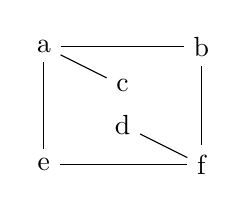
\begin{tikzpicture}
                        [scale=0.5]
                        \node (v1) at (1,10) {a};
                        \node (v2) at (5,10) {b};
                        \node (v3) at (3,9) {c};
                        \node (v4) at (3,8) {d};
                        \node (v5) at (1,7) {e};
                        \node (v6) at (5,7) {f};
                        \foreach \from/\to in {v1/v2,v1/v3,v1/v5,v2/v6,v4/v6,v5/v6}
                        \draw (\from) -- (\to);
                    \end{tikzpicture}
                    \hspace{30px}
                    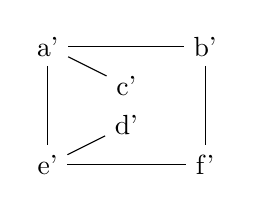
\begin{tikzpicture}
                        [scale=0.5]
                        \node (v1) at (1,10) {a'};
                        \node (v2) at (5,10) {b'};
                        \node (v3) at (3,9) {c'};
                        \node (v4) at (3,8) {d'};
                        \node (v5) at (1,7) {e'};
                        \node (v6) at (5,7) {f'};
                        \foreach \from/\to in {v1/v2,v1/v3,v1/v5,v2/v6,v4/v5,v5/v6}
                        \draw (\from) -- (\to);
                    \end{tikzpicture}
              \item [(iv)] If $G$ and $H$ are isomorphic, then there exists a bijection $f:V(G)\rightarrow V(H)$ such that every vertex $u\in V(G)$ has the same degree as $f(u)$.\\\textbf{Answer: True}, by definition of graph isomorphism; since $\{x,y\}\in G\Leftrightarrow \{f(x),f(y)\}\in H$ for all distinct vertices $x,y\in V$, the corresponding vertices must have the same number of edges connected to it, i.e. $u$ and $f(u)$ have the same degree.
              \item [(v)] If $G$ and $H$ are isomorphic, then there exists a bijection $f:E(G)\rightarrow E(H)$.\\\textbf{Answer: True}; since $G$ and $H$ are isomorphic, by definition, there exists a bijection $f:V(G)\rightarrow V(H)$ such that $\{x,y\}\in E(G)\Leftrightarrow\{f(x),f(y)\}\in E(H)$ for distinct $x,y\in V(G)$.
              \item [(vi)] $G$ and $H$ are isomorphic if and only if there exists a map $f:V(G)\rightarrow V(H)$ such that for any two vertices $u,v\in V(G)$, we have $\{u,v\}\in E(G)\Leftrightarrow\{f(u),f(v)\}\in E(H)$.\\\textbf{Answer: False}, $H$ can contain more vertices than $G$ under this definition.
              \item [(vii)] Every graph on $n$ vertices is isomorphic to some graph on the vertex set $\{1,2,\ldots,n\}$.\\\textbf{Answer: True}, since the graph is isomorphic to itself.
              \item [(viii)] Every graph on $n\geq 1$ vertices is isomorphic to infinitely many graphs.\\\textbf{Answer: True}, since the vertices can be labeled infinitely number of ways.
          \end{itemize}
    \item [4.1.4] Show that a graph $G$ with $n$ vertices is assymetric if and only if $n!$ distinct graphcs on the set $V(G)$ are isomorphic to $G$.\\\textbf{Answer: }
    \item [4.1.6] How many graphs on the vertex set $\{1,2,\ldots,2n\}$ are isomorphic to the graph consisting of $n$ vertex-disjoint edges?\\\textbf{Answer: }
    \item [4.2.1] Prove that the complement of a disconnected graph $G$ is connected.\\\textbf{Answer: }
    \item [4.2.2] What is the maximum possible number of edges of a graph with $n$ vertices and $k$ components?\\\textbf{Answer: } To construct a graph with $n$ vertices and $k$ components with the maximum possible number of edges would be to construct a complete graph with as many vertices as possible, then leave the rest of the vertices as components. In other words, we would have $k-1$ single vertices and a complete graph with $n-k+1$ vertices, which gives us $n-k+1\choose 2$ edges.
    \item [4.3.5] Draw all nonisomorphic graphs with score (6,3,3,3,3,3,3). Prove that none was left out.\\\textbf{Answer: }
    \item [4.3.6] Find an example, as small as possible, of a graph with 6 vertices of degree 3, other vertices of degree $\leq 2$, and with 12 edges.\\\textbf{Answer: } By Prop. 4.3.1, $\text{deg}_G(v)=24$. Then the smallest graph would have 6 vertices of degree 3 and 3 vertices of degree 2.
    \item [P0] Find the number of subgraphs of $K_6$ isomorphic to each of the following: $K_4$, $C_4$, $P_4$, and $K_{2,3}$.\\\textbf{Answer: }\begin{itemize}
              \item [$K_4$:] \textbf{15 subgraphs}; we can get $K_4$ from $K_6$ by removing any two vertices and their connected edges. Since we can choose the edges ${6\choose 2}=15$ number of ways, there are 15 subgraphs.
              \item [$C_4$:] \textbf{45 subgraphs}; we can get $C_4$ from $K_4$ by removing a pair of edges that are not connected to the same vertex. We first remove one random edge (we can choose from any 6), then for each edge there exists exactly one other edge that we can remove. Since the order we remove the two edges does not matter, there are $\frac{6}{2}=3$ ways to remove the pair of edges. Then there exist ${6\choose 2}\cdot 3=45$ subgraphs of $C_4$ in $K_6$.
              \item [$P_4$:] \textbf{180 subgraphs}; we can remove any edge from a $C_4$ graph to get $P_4$, therefore there exists $45\cdot 4=180$ subgraphs.
              \item [$K_{2,3}$:] \textbf{60 subgraphs}; we can remove any vertices and its edges from $K_6$ to get $K_5$ (${6\choose 1}=6$ choices). Then, out of the five vertices, choose two vertices (${5\choose 2}=10$ choices), remove the edges between them and in addition remove the edges between the remaining three to obtain a $K_{2,3}$ graph. Therefore there are $6\cdot 10=60$ subgraphs.
          \end{itemize}
    \item [P1] Let $n\geq 3$ be an integer. The complete bipartite graph $K_{n,n}$ on the bipartite partition $V(K_{n,n})=X\cup Y$, where $X=\{x_1,\ldots,x_n\}$ and $Y=\{y_1,\ldots,y_n\}$ is the graph with edge set $E=\{\{x,y\}\mid 1\leq i,j\leq n\}$. Let $u$ and $v$ be two nonadjacent vertices of $K_{n,n}$.
          \begin{itemize}
              \item [1.] Find the number of paths from $u$ to $v$ of length 2.\\\textbf{Answer: } Since $E=\{\{x,y\}\mid 1\leq i,j\leq n\}$ and $u,v$ are nonadjacent, we must have either $u,v\in X$ or $u,v\in Y$. Suppose $u,v\in X$, then a path of length 2 from $u$ to $v$ would be from $u$ to $y_i$ to $v$, $1\leq i\leq n$. Therefore there are exactly $n$ such paths and the same applies if $u,v\in Y$.
              \item [2.] Same for length 3.\\\textbf{Answer: } This is not possible; assume $u\in X$, then path of length 3 means that $v\in Y$. This contradicts with that $u,v$ must be both in $X$ or both in $Y$ as established in the previous part.
              \item [3.] Same for length 4.\\\textbf{Answer: } Assume $u,v\in X$ (the result is the same for $u,v\in Y$ too by symmetry), in addition let $w\in X$. By part 1 there exists $n$ paths of length 2 between $u$ and $w$. Choose arbitrary path $u\rightarrow p\rightarrow w$, $p\in Y$, we then have $n-1$ options for the third edge to connect to (all $y_i\in Y$ except $p$). Then we have $n-2$ options for the last edge (all $x_i\in X$ except $u$ and $w$). Therefore there are $n(n-1)(n-2)$ such paths.
              \item [4.] Same for length $2m$, where $m$ is some integer $\geq 1$.\\\textbf{Answer: } There are $\frac{n!}{(n-2m+1)!}$ such paths. Proof by induction:\\Base case: $m=1$, we have $n$ possible paths per part 1.\\Inductive step: Assume the hypothesis holds for length $2m$ and assume our path starts at a vertex in $X$ (by symmetry the result also holds if the path starts  at a vertex in Y). Let $P=\{p_1,\ldots,p_m\}\subset X$ be vertices on the path in $X$ and $Q=\{q_1,\ldots,q_{m-1}\}\subset Y$ be vertices on the path in $Y$. To add another 2 length to our path, the first edge can connect to any vertices in $Y\setminus Q$, which contains $n-m+1$ possibilities. The second edge can connect to any vertices in $X\setminus P$, which contains $n-m$ possibilities. Then the new walk of length $2m+2$ has $\frac{n!}{(n-m-1)!}(n-m+1)(n-m)=\frac{n!}{(n-m+1)!}$.\\Therefore there are $\frac{n!}{(n-m-1)!}$ such paths by mathematical induction.
          \end{itemize}
\end{itemize}

\end{document}